\label{sec:chunk_flooding}
\begin{figure*}
  %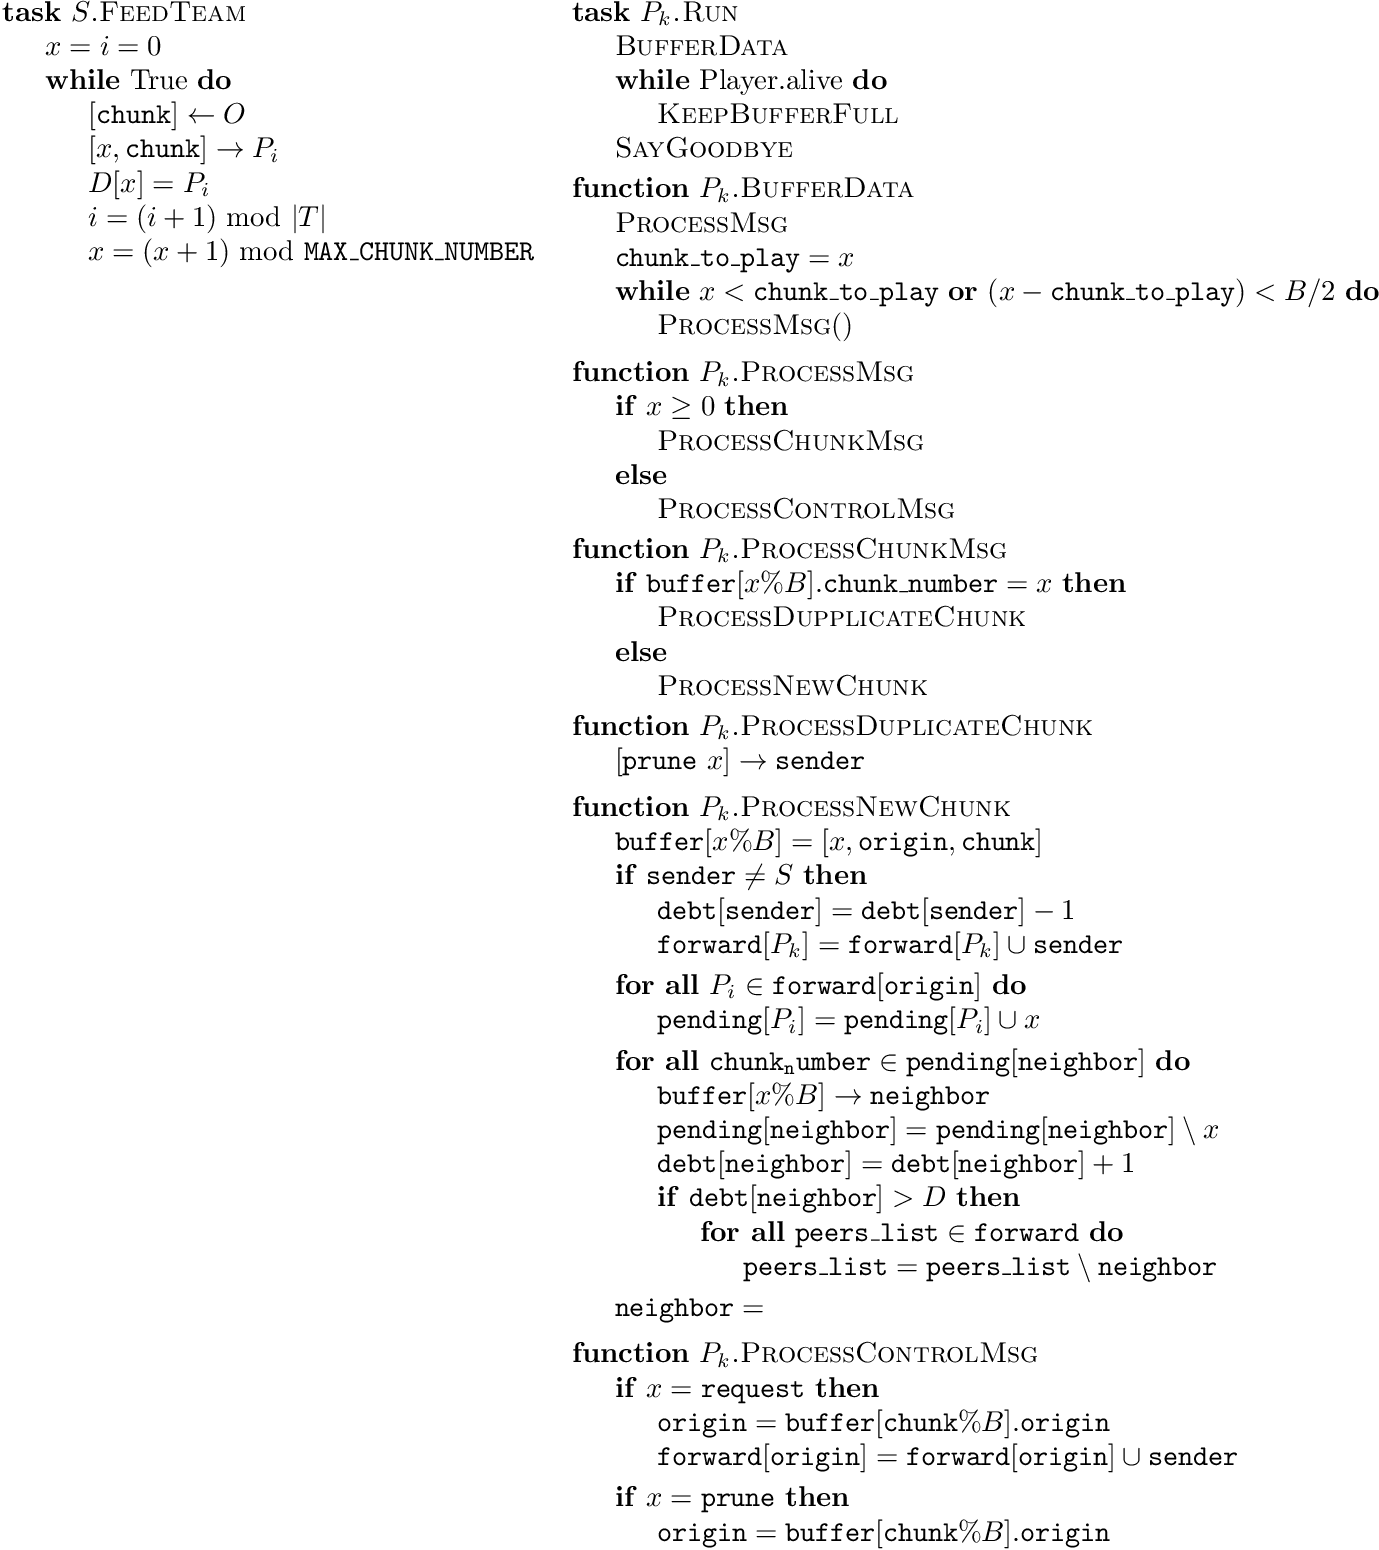
\includegraphics[width=0.75\textwidth]{chunk_generation_and_flooding}
  \fig{300}{3cm}{peer_chunk_flooding}
  \caption{Chunk flooding at peers.\label{fig:peer_chunk_flooding}}
\end{figure*}
When a peer $P_k$ receives a chunk, $P_k$ floods the chunk to each of
its neighbors (except the source), using a prioritized round-robin
schema where those peers with a lower debt are selected first (see
Fig.~\ref{fig:peer_chunk_flooding}). Every time $P_k$ sends a chunk to
$P_l\in T^k$, $P_k$ runs $\mathtt{debt}[P_l] = \mathtt{debt}[P_l]+1$,
and $P_l$ runs $\mathtt{debt}[P_k] = \mathtt{debt}[P_k]-1$. In ideal
circunstances, debs should be $0$. Debs are clipped to $\pm
D$. Obviously, a high supportivity means a low debt, and viceversa.

\begin{comment}
In each round, peers check if a chunk have been received from the rest
of peers of the team (${\cal P}_k\in {\cal T}_j)$). If not, peers send
a $[\mathtt{propagate}~{\cal P}_i]$ to one or more (possibly
to the rest of) peers of the team, where ${\cal P}_i$ is the origin peer
of the missing chunk. At this point, the process continues as
described in Section~\ref{dbs:chunk_flooding}.
\end{comment}

\begin{comment}
For each ${\cal P}_k\in N({\cal P}_i)$, ${\cal P}_i$ checks if a chunk
has been received from ${\cal P}_k$. If ${\cal P}_i$ detects that
${\cal P}_k$ has not sent a chunk to it during $L$ consecutive rounds,
performs $N({\cal P}_i) = N({\cal P}_i)\setminus{\cal P}_k$, and stops
sending to ${\cal P}_k$ more chunks.
\end{comment}
\begin{comment}
computes a
``chunk-debt'', denoted by $d({\cal P}_k)$, that is incremented each
time a chunk is received from ${\cal P}_k$ and decremented each time a
chunk is sent to ${\cal P}_k$. If ${\cal P}_i$ verifies that $d({\cal
  P}_k)>D$ (the maximum debt), then ${\cal P}_i$ considers that ${\cal
  P}_k$ is unable to communicate with it, performs $N({\cal P}_i) =
N({\cal P}_i)\setminus{\cal P}_k$, and stops sending to ${\cal P}_k$
more chunks.
\end{comment}


%When peers receive chunks from their splitter, they must flood them to
%their neighbors until the chunks are broadcasted to the whole team
%(Fig.~\ref{fig:chunk_generation_and_flooding}). Lets suppose that
%${\cal P}_k$ receives a chunk. In the case the sender is its splitter,
%${\cal P}_k$ floods the chunk to $N({\cal P}_k)$. However, if the
%sender is a peer ${\cal P}_m\in N({\cal P}_k)$, ${\cal P}_k$ adds
%${\cal P}_m$ to $N({\cal P}_k)$ if ${\cal P}_m$ is a new neighbor, and
%forwards the chunk to the rest of its neighborhood ${\cal P}_n\in
%N({\cal P}_k)\setminus{\cal P}_m$ if ${\cal P}_k$ is in the shortest
%between ${\cal P}_n$ and the origin peer ${\cal P}_i$ of the relayed
%chunk. This will be true if ${\cal P}_k$ is the gateway of ${\cal
%  P}_n$ to go from ${\cal P}_n$ to ${\cal P}_i$. Therefore, a flooding
%with prunning based on shortest path routing is used.
